\chapter{Semantic Metadata for Open Data Description}
\label{chap:relworks}

In the previous chapter, the issue of building open data skills was tackled through the development of a data literacy course as part of a participatory research.
One of the results of this research pointed out a significant problem related to the organization of ODPs.
Following this motivation, we investigate in this chapter the issue of metadata for open data. 
The chapter is divided in two parts, covering:

\begin{itemize}
	\item A literature investigation over the possible strategies to deal with semantic metadata for organization of open data repositories;
	\item An analysis of the current usage status of metadata in ODPs.
\end{itemize}

Particularly, in the first part we selected works related to semantic enrichment of metadata in ODPs, in order to position the main contribution of this thesis presented in the following chapter.
Section starts with some preliminary discussions regarding semantics and metadata.
Then, a characterization of our contribution is driven, in order to delimit the related research topics.
After this characterization, we present in each section one topic, highlighting the main related works, their gaps and relations to this work.
We start with Assessment of Metadata in \autoref{sec:metadata_assessment}, followed by Metadata Cleanup in \autoref{sec:metadata_cleanup}, Metadata Reconciliation in \autoref{sec:metadata_reconciliation} and finally with Structure Emergence in \autoref{sec:emergence}.

The second section aims to bring light over the current status of metadata usage in Open Data Portals.
Based on the CKAN Census of ODPs, we profile 87 portals and analyse several aspects regarding metadata.
The analysis embraces not only local aspects regarding individual portals, such as use, reuse and similarity within a portal (\autoref{sec:local_metrics}), but also global features between portals, such as coincident metadata and expressiveness (\autoref{sec:global_metrics}).

We conclude in the last section with an evaluation of the literature gaps and the actual problems detected in ODPs, pointing out our strategies to be developed in the next chapter.

\section{Semantic Metadata: A Literature Review}
\label{sec:semantic_metadata}

\subsection{Introduction}

It is unnecessary to argue that good metadata are crucial for making data usable.
By \emph{good} we can give as example a series of quality attributes such as clean, well organized, detailed, complete, accessible, and meaningful.
Intuitively, metadata is meaningful if it brings new information -- meaning -- for data.
If a consumer asks: ``Which bananas do you have?'', and the seller answers: ``The yellow one!'', this is barely meaningful, since almost all types of banana are yellow.
However, if the seller answers: ``I have \emph{Cavendish}, \emph{Gros Michel}, \emph{Latacan}, and \emph{Cambuta}, which one do you prefer?'', there is much more information accessible through the types of bananas, including colour, size, countries of origin, among others.

On the Web context, the way of enhancing the meaning of an object is to connect it to the Semantic Web, through the Linked Open Data Cloud, as detailed in \autoref{sec:LOD}.
This procedure is also called Semantic Enrichment or Semantic Lifting.
\citeonline{Limpens2013} state a series of motivations for semantically enriching tags in the context of folksonomies, considering data generators, data curators and end-users:
\begin{enumerate}
	\item enriching tag-based search results with spelling variants and hyponyms, or 
	\item suggesting related tags to extend the search, or 
	\item semantically organizing tags to guide novice users in a given domain more efficiently than with flat lists of tags or occurrence-based tag clouds, or 
	\item assisting disambiguation.
\end{enumerate}

A more detailed view about problems caused by the absence of semantics in metadata is described by~\citeonline{Marchetti2007}.
According to them, there are six categories of problems:

\begin{citacao}
\begin{enumerate}
\item \textbf{Polysemy:} the same word can refer to different concepts (the word ’field’ can refer to a piece of land cleared of trees and usually enclosed, but also to a branch of knowledge);
\item \textbf{Synonymy:} the same concept can be pointed out using different words (’auto’, ’car’, ’machine’ are three different words that refer to the same concept: a four wheels vehicle);
\item \textbf{Different lexical forms:} the same concept can be referred to by different noun forms, for instance plural nouns (’car’/’cars’), different verb conjugation (’buy’/ ’buying’), name-adjective couple (’energy’/’energetic’), multiple words (’pc’/’personal computer’) and so on;
\item \textbf{Misspelling errors or alternate spellings:} typing errors that occurs when we write a word (’staton’ in place of ’station’) or different possible spelling of the same word (’color’/’colour’);
\item \textbf{Different levels of precision:} the specificity of the word chosen to tag a resource (’jazz’ is more specific than ’music’);
\item \textbf{Different kinds of tag-to-resource association:} implicit kinds of relations that links a tag to a specific resource (’interesting’ expresses an opinion on the resource, ’car’ expresses the topic of the resource and so on) \cite[p.2]{Marchetti2007}.
\end{enumerate}
\end{citacao}

Around ten years ago, discussions about semantifying folksonomies started.
Probably on of the most important work at that time was \emph{Ontology of Folksonomy: a mash-up of Apples and Oranges}~\cite{Grubber2007}.
This work, published first on the web in November of 2005, aimed to clear up a false contradiction between ontologies, as the enabling technology for sharing sharing information on the Semantic Web, and folksonomies, a typical phenomenon of the Social Web representing data emerged from shared information.
It is perfectly reasonable that these two concepts could be understood as contradictory: while ontologies are formally built by domain experts and ontology engineers, folksonomies are freely constructed by users.
After clarifying the role of each concept, Grubber defines the ontology of folksonomy, whose central element is \emph{Tagging}, which is an activity involving an object $O$, an user $U$, a tag $T$ and a system $S$.
The possibility of qualifying a tagging is also mentioned, for example, as a negative tagging.

Another important work introducing this topic is \emph{``Ontologies are us: A unified model of social networks and semantics''} \cite{Mika2007}, also published first in November of 2005.
Mika also disagrees that ontologies and folksonomies are contradictory, but differently from Grubber, for who both are distinct concepts (Apples and Orange) that can be united, he states that ``folksonomies are ontologies''.
In order to justify it, author cites a set of broad ontology definitions, and classifies folksonomies in these definitions as ``lightweight, dynamic and limited in sharing scope''.

In the sequence of these papers, several authors tried to define tagging ontologies.
\citeonline{Wu2006} added a time dimension to the tagging model.
And to the best of our knowledge, \citeonline{Newman2005} was the first to propose an ontology for tagging.
This work was further extended by \citeonline{Knerr2006}, who proposed the Tagging Ontology, depicted in \autoref{fig:tagging_ontology}.
All dimensions proposed by \citeonline{Wu2006} and \citeonline{Grubber2007} are present and further detailed in this ontology.

\begin{figure}[b]
\begin{center}
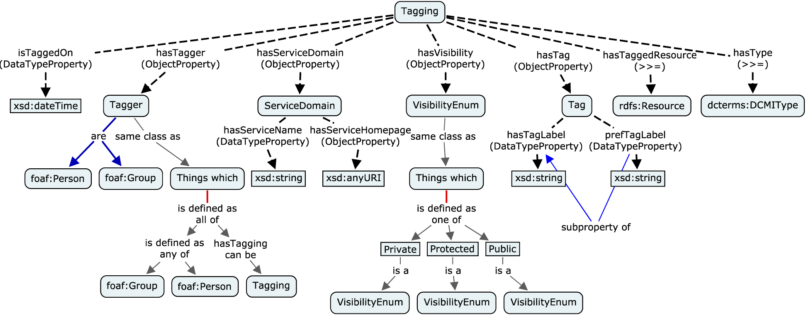
\includegraphics[width=\columnwidth]{images/tagging_ontology.png}
\caption[Tagging Ontology.]{Tagging Ontology. Source: \citeonline{Knerr2006} }
\label{fig:tagging_ontology}
\end{center}
\end{figure}

Although crucial, these models are not complete enough to solve problem of creating ontologies emerged from collaborative tagging.
\citeonline{Halpin2007} analysed the dynamics of collaborative tagging, in order to determine the possibilities of extracting knowledge.

It is important to notice that until this point, tagging ontologies were concerned with organizing the knowledge contained in the tagging activity.
The MOAT architecture was the first to explicitly include the concept of tag meaning, associating each tagging element to a LOD resource~\cite{Passant2008}.

A review about semantic tagging initiatives by \citeonline{Kim2008} compared the different types and relations proposed by the works until 2008, and was updated by \citeonline{Kim2011}.
The most recent attempt to build a tag ontology is the Modular Unified Tagging Ontology (MUTO)\footnote{\url{http://muto.socialtagging.org/core/v1.html}}, shown in \autoref{fig:muto}, and described by~\citeonline{Lohmann2011}.
It incorporates suggestions of several previous models into a unified model, and is strongly based on wide used ontologies, such as Dublin Core, SKOS and SIOC. 

\begin{figure}[b]
\begin{center}
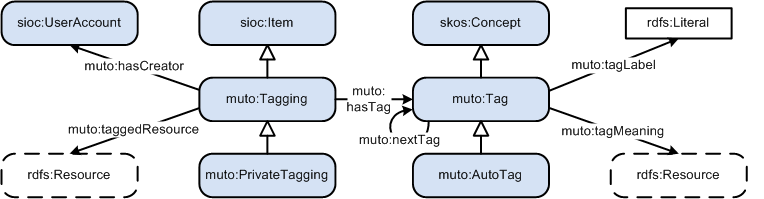
\includegraphics[width=\columnwidth]{images/muto.png}
\caption[MUTO Ontology.]{MUTO Ontology. Source: \citeonline{Lohmann2011}}
\label{fig:muto}
\end{center}
\end{figure}

Finally, in the context of tagging semantics, it is also important to discuss the nature of the relation between tags and tagged resources.
To the best of our knowledge, none of the proposed tagging ontologies incorporates the possibility of qualifying this relationship.
\citeonline{Marchetti2007} point out the question of ``implicit kinds of relations that links a tag to a specific resource'' with an example: ``\emph{interesting} expresses an opinion on the resource, \emph{car} expresses the topic of the resource.''

\subsection{Characterization of the Contribution}

The main contribution of this thesis is a semantic approach for organizing metadata in Open Data Portals, specifically regarding tags.
Thus, the following topics are considered to be related works, and will be analysed in the following:
\begin{itemize}
	\item Metadata assessment: how to assess the use and quality of metadata;
	\item Metadata clean-up: how to enhance the quality of the metadata using strategies such as spell-checking, detection of similar words, special characters equalization, and others;
	\item Metadata reconciliation: how to align metadata with standard vocabularies, thesauri and ontologies;
	\item Structure emergence: how find semantic relation between metadata.
\end{itemize}

Regarding the related bibliography, it is necessary to highlight that the vast majority of scientific works about tagging and semantics focus on a different context in relation to ours.
It is normally assumed a folksonomy environment, where tags are attributed to resources by the crowd, passing through a crowd-selection mechanism, which may enhance the tagging quality, but can also insert some inherent noise.
This is applicable to platforms such as del.icio.us of flicker, where several users can tag the same resource.
However, in the open data portals context, tags are only attributed by system managers.
Although less noisy, this procedure is biased by few taggers.

In the following subsections, we analyse the literature contributions regarding the above cited topics in relation to our work.

\subsection{Metadata Assessment}
\label{sec:metadata_assessment}

An important step in working with metadata is to develop methods for evaluating quality aspects of it.
\citeonline{Reiche2013} implemented quality metrics for metadata in ODPs which can be assessed automatically.
In this work, authors measured completeness, weighted completeness, accuracy, richness of information and accessibility as defined by \citeonline{Ochoa2006}.
Although the metrics definition are significant, their implementation in an automatic context is simplified, which in practice turns the accuracy and richness of information, for example, very weak.

In relation to the metrics for tagging environments, some related ideas could be found in the literature.
For example, \citeonline{Umbrich2015} present a framework to evaluate the quality of ODPs. 
Among the applied quality metrics, three of them -- \emph{Usage}, \emph{Completeness} and \emph{Accuracy} -- are related to metadata keys, which tags are part of. 
\emph{Usage} establishes which metadata keys are actually used in a portal; \emph{Completeness} evaluates the presence of non empty values; and \emph{Accuracy} checks if metadata adequately describes the data.
This metric, however, is not applied for tags.

Laniado and Mika did a similar analysis over hashtags on Twitter~\cite{Laniado2010}.
Their work is focused in answering if Twitter hashtags constitute \emph{strong identifiers} for the semantic web. 
To achieve this, four metrics are used: frequency of hashtags; specificity, which is the deviation from the use of them without being a hashtag; consistency; and stability over time.

\citeonline{Colpaert2014} presented a method for calculating interoperability between ODPs based on  identifiers used in datasets.
These identifiers are unique identifications for datasets, and process of considering them equal or different is manual.
The metric takes into account if the same identifiers were used to represent the same concepts in a dataset, and then calculates an interoperability metric.

These works are taken into account in \autoref{sec:analysis}, where we derive an extensive analysis over ODP metadata.

\subsection{Metadata Clean-Up}
\label{sec:metadata_cleanup}

When dealing with metadata of large datasets, a cleaning up procedure is usually the first step before start working with it.
There are several strategies for cleaning up tags described in the literature.

\citeonline{Angeletou2008}, in a context of semantic enrichment of folksonomy tagspaces, describes a Lexical Processing procedure to clean-up tags containing special characters, numbers, concatenated tags or tags with spaces.
Two steps are proposed in this work: the first is called Lexical Isolation, which uses a set of heuristics to determine if tags have potential to become semantic identifiers.
The following step is called Lexical Normalisation, which aims to produce a list of possible lexical representations for each tag, considering plural and singular forms, different verb tenses, and others.

Although the focus of \citeonline{Specia2007} lies on creating tags clusters, their procedure to integrate folksonomies to the semantic web also includes a pre-processing phase.
As in the previous work, the first step consists in removing tags with low chances of being mapped in an ontology.
In the sequence, a series of heuristics are used to group morphologically very similar tags, including the Levenshtein distance.
In order to choose the more significant tag in a group, preference is given to words that can be found in the WordNet base.
The last step of the cleaning procedure is to eliminate tags with a low frequency, or appearing only in an isolated form.

In the context of library metadata, \citeonline{VanHooland2013} describes as a first step for metadata reconciliation ``profiling and cleansing of metadata''.
Using an open source tool, authors describes cleaning activities such as deduplication (remove duplicate entries), atomization (explode overloaded fields), applying facets and clustering.


\subsection{Metadata Reconciliation}
\label{sec:metadata_reconciliation}

On the metadata context, reconciliation refers to the process of finding a correspondence for some text string in a controlled vocabulary, thesaurus or ontology.
To the extent of our problem, we are going to analyse strategies for mapping possible multi-language tags into defined ontologies, in order to be able to semantically process these tags.

The reconciliation approach described by \citeonline{VanHooland2013} consists simply in searching the categories in pre-defined ontologies such as Library of Congress Subject Headings (LCSH) and Powerhouse Museum.
This approach is followed by some content specific processing in order to equalize plurals. 

\citeonline{Lawler2012} developed the Open Reconcile tool, a reconciliation tool tailored to help metadata curators to ensure the compliance of datasets with controlled vocabularies.
Alongside the automatic procedures, user are allowed to build a synonym table in order to provide manual input to the algorithm.

A whole Semantic Tagging system is proposed by \citeonline{Marchetti2007}.
The system, implemented as a browser plugin, allows users to tag web resources and choose a corresponding semantic resources from knowledge bases such as Wikipedia.

As we can see, several conventional approaches do not include any semantic intelligence on the reconciliation task.
This is not the case of the technique described in \citeonline{Angeletou2008}.
In this case, author first performs a sense disambiguation, which consists of calculating the similarity distance to co-occurring tags, and then select the sense with the smaller distance.
This procedure is deeper detailed in \citeonline{Angeletou2008a}.
The second step is called Semantic Expansion, which is justified by the sparseness of the Semantic Web.
In this step, synonyms and synonyms of the hypernyms of the correct sense are included in order to search for semantic web entities (SWE).
The process is finalized by searching for SWEs in the Watson\footnote{Available at \url{http://watson.kmi.open.ac.uk/WatsonWUI/}.} platform, and choosing the most adequate according to the defined criteria.

Instead of grouping tags using semantic criteria, \citeonline{Specia2007} use a statistical approach for this.
An $N \times N$ co-occurrence matrix is built, where $N$ is the number of distinct tags, and each element $m_{ij}$ represents the number of times that tags $i$ and $j$ co-occur in different resources.
Thus, the lines or columns of this matrix are vectors representing the tags, and the angular distance between them are calculated in order to cluster the closer tags.
After building the clusters, terms are pairwise searched in ontologies in order to find the appropriate semantic entity.
This procedure is also used for finding relations between the tags, which will be discussed in the following section.

%http://pt.slideshare.net/Freddy.Limpens/phd-defense-multipoints-of-view-semantic-enrichment-of-folksonomies

\subsection{Structure Emergence}
\label{sec:emergence}

Finding semantics entities related to tags is an important step.
However, in order to build a knowledge base, it is necessary to find and qualify relations between these entities.
Some of the above cited works also proposed strategies for this step.

\citeonline{Specia2007} searches if a pairs of tags appears on the same ontology, and in case of success, relations are extracted directly from the ontology.

Several approaches described on the literature make use of similarity measures in order to determine the relation between two tags.
The topic of similarity measures is very extensive, and several strategies can be found on the literature \cite{Harispe2015, Harispe2014, Trillo2007, Cilibrasi2007}.
A number of works, such as \cite{Limpens2013}, use the WordNet database in order to determine the relation between two words.
The hierarchical structure of WordNet allows to determine broader and narrower relations, as well as to calculate the distance between words through the WordNet tree.
It is worth highlighting a paper by \citeonline{Cattuto2008}, where several measures of relatedness are compared to WordNet similarity in the context of tags in social bookmarking systems.
Relatedness is considered to be a special case of similarity, which is grounded only in the folksonomy (and not in external sources, as in \citeonline{Angeletou2008}).
The alleged reason for grounding the measures only in the folksonomy is the use of community specific terms, which may not be present in external vocabularies.
\citeonline{Cattuto2008} presents three groups of relatedness measures: co-occurrence, distributional measures and FolkRank, which uses a similar approach as the PageRank algorithm.

A very interesting point-of-view on this topic is brought by \citeonline{Limpens2013}.
In this work, a complete model for the semantic enrichment of folksonomies is presented including a socio-technical approach for managing diverging points of view, e.g., ``Kevin agrees with the fact that soil pollution is a more specific term than pollution but Alex disagrees''.
\autoref{fig:srtag} shows the proposed model.
After driving an automatic reconciliation and structuring strategy, which is then validated or corrected by users, the divergences are managed by a conflict solving module.

\begin{figure}[h]
\begin{center}
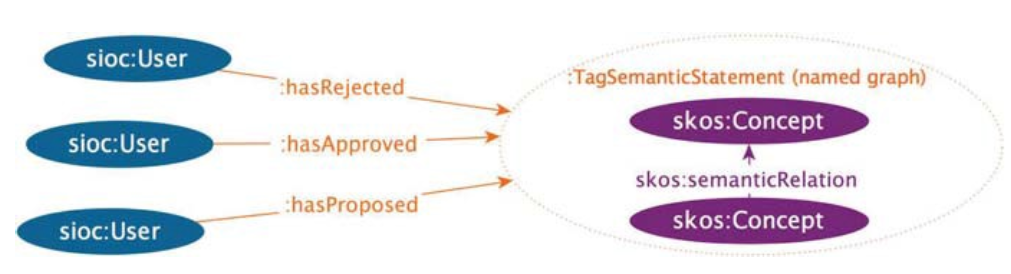
\includegraphics[width=\columnwidth]{images/SRTag.png}
\caption[SRTag RDF schema.]{SRTag RDF schema. Source: \citeonline{Limpens2013}}
\label{fig:srtag}
\end{center}
\end{figure}

\subsection{Automatic Semantic Tagging}
\label{sec:automatic_semtags}
Although this is not the main objective of this work, it is worth mentioning some strategies for automatic semantic tagging of documents.
\citeonline{Allahyari2016} proposes a probabilistic model based on DBPedia hierarchical model to automatically determine categories to documents.
The model was successfully tested on a Wikipedia sample and on a Reuters database.
Since categories are DBPedia resources, they can be considered as semantic metadata for linking purposes.

\citeonline{Chemudugunta2008} proposes a similar approach, but using unsupervised statistical learning.
The generic model can be used both with human-defined concept and data-driven topics, and was tested against an educational text corpus.

\subsection{Semantic Lifting in ODPs}
The problem of semantic lifting in ODPs was tackled by~\citeonline{Ermilov2013} and \citeonline{Ding2011}. 
In~\citeonline{Waal2014}, a strategy for lifting datasets in ODPs to the Linked Data cloud is presented. 
In all these works, however, the semantic lifting refers to the datasets, and not to metadata.

%#########################################################################################
\section{An Analysis of Metadata in ODPs}
\label{sec:analysis} 
%#########################################################################################

Besides having an overview about literature related to semantic metadata, it is also necessary to the proper development our work to profile the use of metadata in Open Data Portals.
In order to propose innovations, it is mandatory to know the main problems of real-world metadata usage.

In this section, we profile the use of metadata in Open Data Portals, with a special focus on tags. 
The analysis is restricted to systems running CKAN\footnote{Available at \url{http://ckan.org}}, the standard open-source software for ODPs. 
The CKAN community publishes a census\footnote{Available at \url{http://ckan.org/instances}}, where 139 portals were listed at the time of the experiment. 
Through the API offered by CKAN, we tried to obtain data from all portals, but only 87 responded adequately when the assessment was performed (March of 2016).
Reasons for the lack of availability were mainly that the portal was completely offline, the API was disabled or not responding at the same URL of the website or the portal was using an outdated version of CKAN.

The majority of ODPs is related to governments and public administrations at local, regional, national or continental levels. 
Some of them are also focusing on specific themes, such as energy or geothermal data. 
Although most portals are authoritative and run by governments and public administrations, some of them were built as civil society initiatives.
A complete list of the analysed ODPs is available online\footnote{\url{http://bit.ly/1NGygtk}}.

%min_datasets: 4
%max_datasets: 194592
%min_tags: 8
%max_tags: 59208
	
The analysed ODPs are quite heterogeneous. 
The number of datasets in each portals varies from 4 to 194,592, and the number of tags, from 8 to 59,208.
Regarding the quality of the portals, although there is no general benchmark, \emph{\href{http://opendatamonitor.eu}{Open Data Monitor}} attests a high heterogeneity within European ODPs.
An informal quality assessment using the Five Stars of ODPs~\cite{Colpaert2013} also shows that portals vary from simple data registries (one star) to a common data hub (five stars).

A summary of the experiment data is shown in \autoref{tab:summary}. 
The code used to collect and analyse the data is available as an open-source project\footnote{\url{https://github.com/alantygel/StodAp}}.

\begin{table}[]
\centering
\ABNTEXfontereduzida
\caption{Summary of data used in the experiment.}
\label{tab:summary}
\begin{tabular}{l|c}
Portals & 140 \\
Analysed Portals & 87 \\
Tags & 290,075 \\
Groups & 1,701 \\
Datasets & 470,551 \\
Datasets without group & 417,393 \\
Datasets without tag & 172,157 \\
\end{tabular}
\end{table}

%%\begin{savenotes}
%\begin{table}[tb]
%\caption{Summary of data used in the experiment.}
%\label{tab:summary}
%\begin{center}
%\begin{tabular}{l|c}
%Portals & 90 \\
%Datasets & 	389,913 \\
%Overall tags & 220,567 \\
%Unique tags & 148,657 \\
%Average tags per portal & 2451 \\	
%Average tags per dataset & 3.88 \\	
%Association with semantic resources & 36\% \\
%Groups & 1500 \\
%Average groups per portal\footnote{Excluding ODPs which do not use groups.} & 21.43 \\
%Average datasets per group\footnote{Excluding void groups.} & 67.45 \\
%\end{tabular}
%\end{center}
%\end{table}
%%\end{savenotes}

The analysis is divided in two groups: local metrics, to analyse the quality of tags in a particular ODP, and global metrics, looking at the interrelations between portals, and with the Linked Open Data (LOD) cloud.

Regarding the other main tool for organizing ODPs -- groups -- \autoref{tab:summary} also shows the number of groups per portal, and the number of datasets inside each one.
While the tags are attributed to an average 3.88 datasets, groups contain a mean value of 67.45 datasets.
This makes groups less selective than tags, which justifies our decision to focus on tags in this work.
Moreover, while all 87 portals use tags, 18 do not use groups to organize data.

In the following, we present the metrics and their results divided into Local Metrics, i.e., applied separately to each portal, and Global Metric, where a joint analysis is driven.
First ones aim to assess the use of tags and verify enhancement possibilities, and the last ones assess the viability of using tags as main elements of communication between portals.

\subsection{Local Metrics}
\label{sec:local_metrics}

\subsubsection{Tag Reuse}
The objective of this metric is to assess whether a single tag is being used to characterize several datasets, just a few or even only one.
Creating new tags for each dataset can be considered a bad tagging practice.
If tags are reused for several datasets, tag-based information retrieval will be more effective.
\autoref{fig:tags_once} shows the distribution of the percentage of tags used only once for each portal. 
The graphic shows a peak around 70\% of the tags used only once.
From the 87 portals, 75 use more than 50\% of the tags only once.
As a conclusion, tag reuse can be considered very low, thus effectively preventing the tags to be a suitable means to improve navigation, exploration and retrieval of datasets from ODPs.

%add examples
%include std and mean

\begin{figure}[tb]
\begin{center}
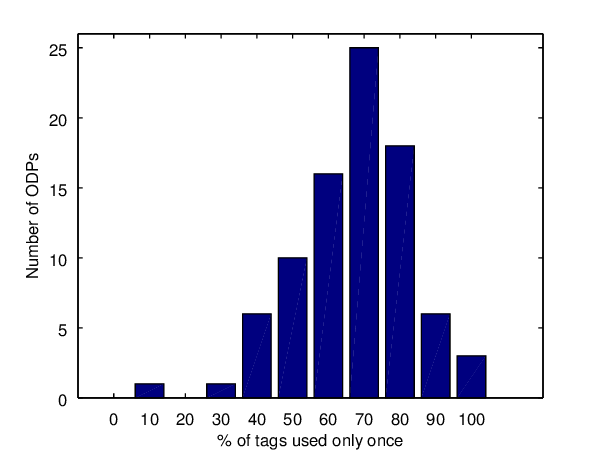
\includegraphics[width=\columnwidth]{images/tag_once_dist.png}
\caption[Re-use of tags inside an ODP.]{Re-use of tags inside an ODP. The graphic shows the distribution of the percentage of tags used only once.}
\label{fig:tags_once}
\end{center}
\end{figure}

\subsubsection{Tags per Dataset}
This metric assesses the number of tags used per dataset.
%rephrase
The goal is to verify, as in~\citeonline{Umbrich2015}, if the tag metadata is being actively used in the portals.
We must note that the results of this metric cannot lead to further conclusions, since we do not intend to define an optimal value for the number of tags per dataset. 
Using few and consistently used tags may support the organization of datasets better than many incoherently used ones.
On the other hand, few tags may not label the content adequately.
\autoref{fig:tags_per_ds} shows the distribution of the average tags per dataset for each portal. 
We can see that most ODPs apply between 1 and 7 tags to each dataset, with a peak around the value of 3.
In general, we can affirm that describing datasets with tags is a common procedure in ODPs.

\begin{figure}[tb]
\begin{center}
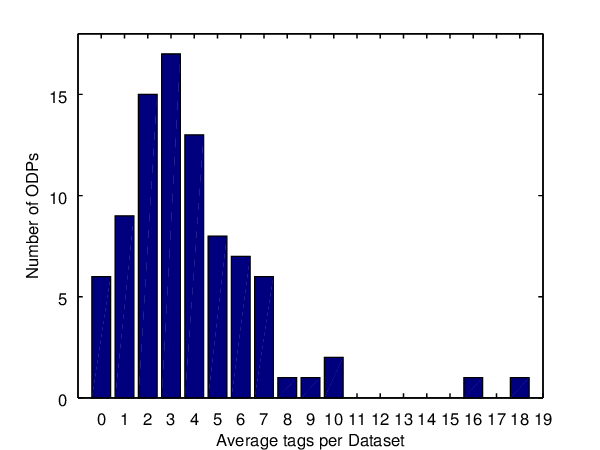
\includegraphics[width=\columnwidth]{images/tags_per_dataset.png}
\caption[Average number of tags per dataset.]{Distribution of the average number of tags used per dataset in ODPs.}
\label{fig:tags_per_ds}
\end{center}
\end{figure}

\subsubsection{Tag Similarity}
By looking at the ODP tags, one can readily recognize that many tags differ only on capitalization, accents or singular and plural forms.
Thus, this metric assesses whether several tags are being used with the same meaning.
While recognizing these cases is easy for humans who understand the language of the tags, an automatic discovery of tags with the same meaning is not always straightforward.
A simple approach is to convert the tags to lowercase and unaccented strings for comparison. 
Despite its simplicity, this method catches a significant number of cases such as \texttt{birth} and \texttt{Birth}.

A second possibility is to use the well known Levenshtein edit distance, which can also be suitable for detecting gender and plural differences, in some languages. 
This algorithm calculates the minimum number of character modifications -- insert, delete and edit -- necessary for turning a sequence into another. 
However, this method fails with tags containing numbers. 
For example, the Levenshtein edit distance between \texttt{budget-2010} and \texttt{budget-2011} is the same as between \texttt{Access} and \texttt{access}.
Semantic-oriented methods, as detailed in~\citeonline{Harispe2015}, could also be used to detect synonymous tags.

For our purposes, we define similarity as:

\begin{equation}
	S = \frac{\textrm{Similar Pairs}}{\textrm{Number of Tags}} * 100,
\end{equation}
where Similar Pairs is the number of tag pairs where tags are equal after lowercasing and unaccenting.
\autoref{fig:similarity} shows the distribution of similar tags inside each ODP.
% Similarity was checked using the simple approach.
The occurrence of a significant rate of similarity reveals that there are few portals adopting a systematic tagging procedure.
Despite the low percentage for some portals, in many of them similar tags still occur.
Only 20 portals, out of overall 87, revealed no similar tags at all. 
It should be noticed that these portals use far less tags (average 148 per portal) than the global average of 2451 per portal, which may also be a sign of careful tagging.

\begin{figure}[tb]
\begin{center}
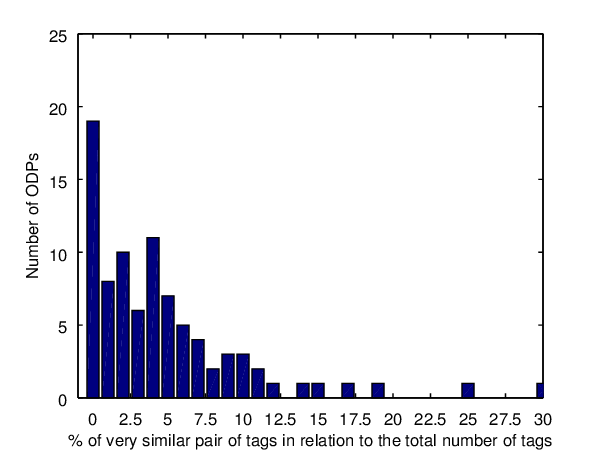
\includegraphics[scale=1.2]{images/similarity.png}
\caption[Percentage of very similar tags in ODPs.]{Percentage of very similar tags in ODPs, where the difference lies only in capitalization or special characters.}
\label{fig:similarity}
\end{center}
\end{figure}


% TODO make clear that it is only the 

\subsection{Global Metrics}
\label{sec:global_metrics}

\subsubsection{Coincident tags between portals}
Different ODPs, especially governmental ones, can publish related data, which may also be tagged similarly.
A similar measurement was used by \citeonline{Umbrich2015}.
Using the same tag comparison approach as described in the local tag similarity metric, we found that 79,882 tags appeared in more than one ODP, which represents 28\% of the total tags. 
This figure, however, should be carefully analysed. 
If we are interested in datasets from different ODPs tagged similarly, an overestimation bias may come from the fact that some portals act only as datasets harvesters, replicating the same datasets (and related tags). 
On the other hand, because portals are available in several languages, different tags could have the same meaning in different languages, what in turn tends to be an underestimation bias.
In any case, the figure clearly indicates that there exists great potential for linking tags between open data portals.
In fact, with this metric, our aim is to justify and motivate the development of a semantic tag curation approach for open data portals, which will be described in \autoref{chap:tagging}. 
%note about context: it do not make sense to compare tags between portals of different contexts
%calculate more than twice

%    Round Number: 1
%    Number of ODPs green: 87
%    Number of ODPs yellow: 1
%    Number of ODPs failled: 51
%    Number of tags: 290075
%    Number of unique tags: 210193
%    Number of datasets: 470551


\subsubsection{Tag expressiveness}
A way of taking the tagging process one step further is to associate tags with resources or terms openly described in knowledge bases.
\citeonline{Passant2008}, while building the MOAT ontology\footnote{\url{http://muto.socialtagging.org/mirror/moat.rdf}}, designed the association of tags with meanings, represented by one or more URIs in the LOD cloud.
With this expressiveness metric, our aim is to check if a tag is suitable to be connected to the LOD cloud, i.e., if there are candidate resources to represent its meaning.

Several knowledge bases are available on the Web, with DBpedia and WordNet being the most prominent ones.
They are characterized by providing both a model of data organization -- ontology -- and the individual instances.
DBpedia\footnote{\url{http://wiki.dbpedia.org/}} is build after Wikipedia knowledge base, and contains more than 38 million things, described in 125 languages using DBPedia Ontology.

WordNet \cite{Fellbaum1998} is one of the most used lexical database for the English language.
Its strengh relies on synsets describing the semantical relations between several senses of words.

In our tests for matching tags with semantic resources, we found that \url{Lexvo.org}~\cite{Melo2013}, was the better service to search connections to different semantic knowledge bases, in several languages.
Lexvo.org is connected not only to Wikipedia and WordNet, but also to Gemet, Wikitionary, Eurovoc, Agrovoc, OpenCyc and others.
By providing an isolated term (in our case, the tag) and its language, Lexvoc.org returns the corresponding translations, as \texttt{lexvo:translation}, and if the term is English, it returns semantic resources, either as \texttt{rdfs:seeAlso} or \texttt{lexvo:means}.

\autoref{tab:expressiveness} shows the results. 
The majority of tags (68.38\%) did not correspond to any semantic resource according to this method.
8.15\% of the tags were not evaluated either because they contain numbers, or because their length was equal or smaller than three. 
In those cases, results are mostly wrong.
For 23.46\% of the tags, at least one meaning or equivalent term was found, and their use represent a similar magnitude of 23.71\%.
Some tags can return several meanings, such as \texttt{leaves}\footnote{\url{http://www.lexvo.org/page/term/eng/leaves}}, for example: abandoning something, handing something to someone, or the plural of leaf, among others. 
In those cases, a further disambiguation procedure is needed.

\begin{table}[]
\centering
\caption[Expressiveness of tags.]{Expressiveness of tags. Percentage of main tags that could be associated to semantic resources. The tag universe considered here refers to clean tags, as described in \autoref{sec:local_building}, and represents 60.58\% of overall tags.}
\label{tab:expressiveness}
\begin{tabular}{|l|c|c|}
\hline
                            & \textbf{Absolute Occurrence} & \textbf{Weighted by Usage} \\ \hline
Associated to a meaning     & 26.35\%           & 36.06\%                    \\ \hline
Not associated to a meaning & 73.65\%           & 63.94\%                    \\ \hline
\end{tabular}
\end{table}

%Tags: 290093
%Main Tags: 175738
%Tags With meaning: 46317
%Tags With meaning weigted: 591429
%Tags With no meaning weigted: 1048636


It is not possible to guarantee that all associations were meaningful, and even worse, that the meaning intended by the tagger was correctly captured.
The tag language was estimated by the ODP locale metadata, which can also be a source of errors if not correctly set.
Some portals are also multi-language, and this characteristic is normally described.
Further evaluations are needed in order to estimate the potential that ODP tags have to be connected to the LOD cloud.
However, we see that at least one fifth of the tags correspond directly to a semantic resource.
Providing context and a stemming pre-processing would probably enhance this result.
Thus, we can say that some semantic potential is present on the tags.


\section{Conclusions}

In this chapter, a theoretical and practical analysis about metadata and tagging in ODPs was driven.
After a general overview on semantic tagging, a literature revision regarding metadata assessment, clean up, reconciliation and relationship presented the recent advanced of metadata curation in relation to the Semantic Web tendency.

Apart from the literature review, looking at the actual use of tags in ODPs was also necessary.
An analysis of 87 ODPs revealed that: (i) tags in ODPs are widely used, but in a non-systematic way, which hinders their capacity of supporting information retrieval, and (ii) there is a potential for using these tags as connecting elements between ODPs, and for raising semantics from them.
Next, we describe our proposal based on these statements.

Ideas and gaps noticed on the literature, and actual problems and potentials detected on ODPs are the basis for proposing the STODaP approach that will be described in the following chapter.

%metadado, extração, muito breve, uma vez tendo tags, o que eu faço para melhorar
%bernardo azevedo tentando pegar localização de tweets - "teoria da mutua informação", tentando descobrir o que está fortemente relacionado e o que não está relacionado. Bons resultados
% tem que ir afunilando para semantica


%% justificativa do capitulo 3: abordagem semi-automatica, puxando para o lado da colaboração
%% imaginar que o processo da descoberta de links tem uma parte automática, mas uma parte de participação dos usuários.
%% viu bastante isso em trabalhos recentes, um deles foi o projeto final da karen na parte de extração semântica de texto, extraindo relações da wikipedia. dado que a dbpedia so pega relações do box, foram para o texto e tentaram extrair e selecionar fatos sobre esse objeto, para complementar a dbpedia . 
%% extração de ontologia a partir do texto, tira as triplas do texto e pede para um usuário validar.
%% joao trabalho bem na parte da relações - 1o identifica as entidades

%% dado que eu to tentando entender, será que eu consigo ter uma mediação para enriquecer com feedback do humano, tanto com especiliastas de domínio qto com usuários

%% usar os usuários na validação do que é automático!!!

%já tentaram descrever melhor, assim assim assado - e os gaps
%(metadata) semantic enrichment 

%Mutual information - o que é mais significativo em um grupamento, que o faz diferente do outro - explorar ligações entre elementos 

%qual a relação do datasem a tag?

